\pagebreak

Block name: Hyst\_diff

Number of inputs: 1

Number of outputs: 1

Parameter list: number of blocks, Hyst\_diff\_ota1\_ibias

Block description: 
A vectorized hysteric differentiator. It implements the most basic property of time derivative which is that changes in input signal are amplified, whereas the steady value of the input signal is not. 
It is achieved by a single amplifier with a nonlinear element in the feedback path shown in the figure. 
The large signal behaviour of this circuit follows following equations
For increasing input voltages
\begin{equation}
V_{out} = \kappa V_c + ln(\frac{C dV_c/dt}{I_o})
\end{equation}
For decreasing input voltages
\begin{equation}
V_{out} = \kappa V_c - ln(-\frac{C dV_c/dt}{I_o})
\end{equation}
For more detailed explanation on this read chapter 10 of Analog VLSI and Neural Systems book by Carver Mead.

\begin{figure}[H]  % jpg, png, or pdf
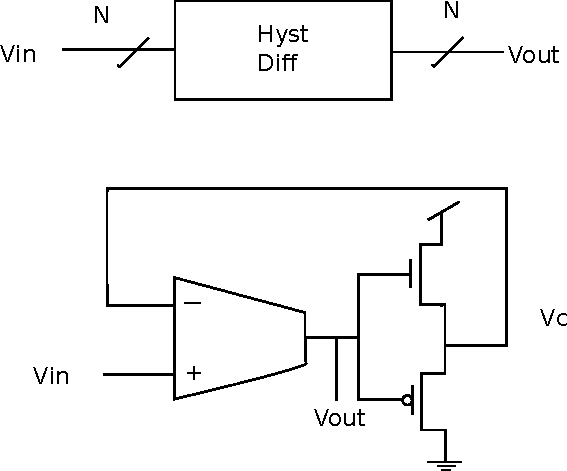
\includegraphics[width=300pt]{/home/ubuntu/rasp30/sci2blif/documentation/blocks_latex/figures/Hyst_diff.pdf}
\end{figure}

